% features selection description for the prediction problem (this is EDA) - here you should select most interesting features relevant for the specific type of application type using for the simplest case correlation coefficients
% EDA of selected features - here you should try to analyze the dependence of the features on the target value (the deans decision)

At the beginning a pairplot was created from all features to find some correlations. When there is so many features it is hard analyze it but it helped to select not correalted features. Drawing the image was time consuming due to the number of the columns. The result was drawn as Fig.~\ref{fig:all_features_pariplot}. It is possible to observe that 'missing\_ECTS' and 'ECTS\_in\_recent\_semester' are corelated.


\begin{figure}
    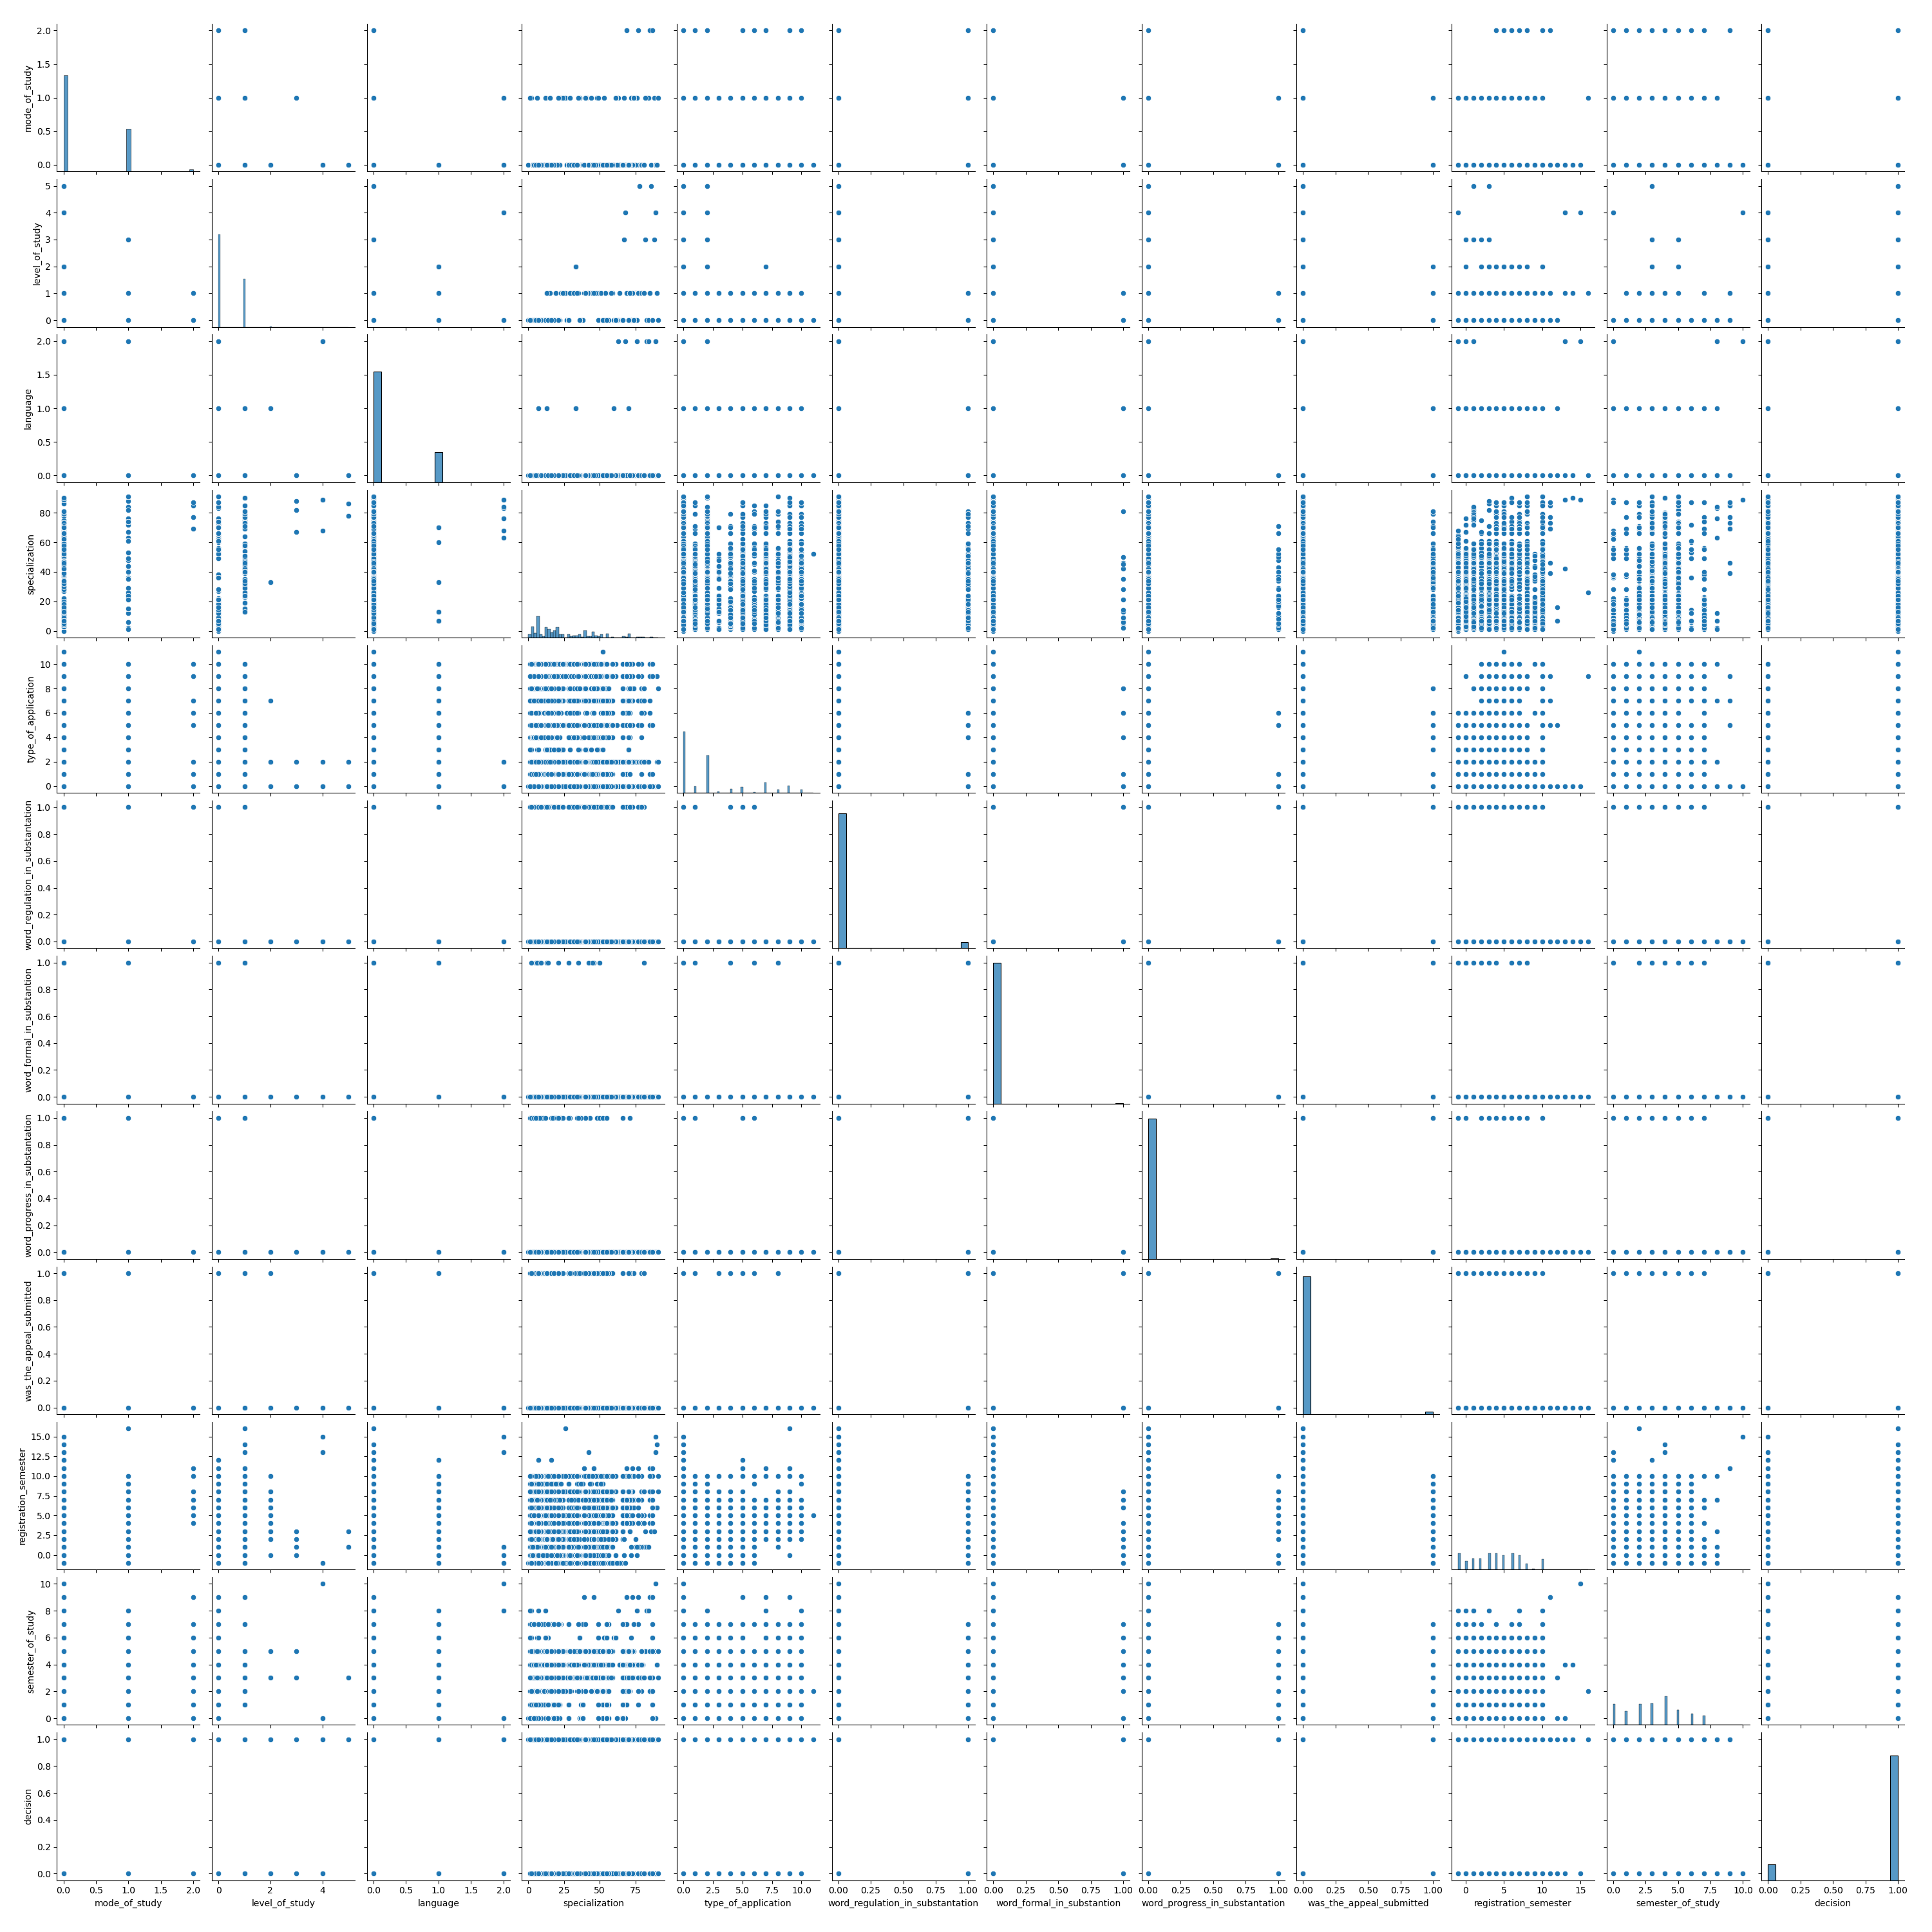
\includegraphics[width=0.5\textwidth]{img/pairplot.png}
    \caption{Pairplot of all columns in dataset}
    \label{fig:all_features_pariplot}
\end{figure}


Then there was selected six features using the column names and intuition. The selected features was presented in the table~\ref{tab:selected_features}. The pairplot for the features is visible at Fig.~\ref{fig:selected_features_pariplot}.
"mode\_of\_study", "level\_of\_study", "specialization", "type\_of\_application" are categorical columns with limited possible option. "semester\_of\_study" and "missing\_ECTS" have discrete values. In figures ~\ref{fig:box_missing} and ~\ref{fig:box_semester} there are boxplots of values in columns "semester\_of\_study" and "missing\_ECTS".

\begin{figure}
    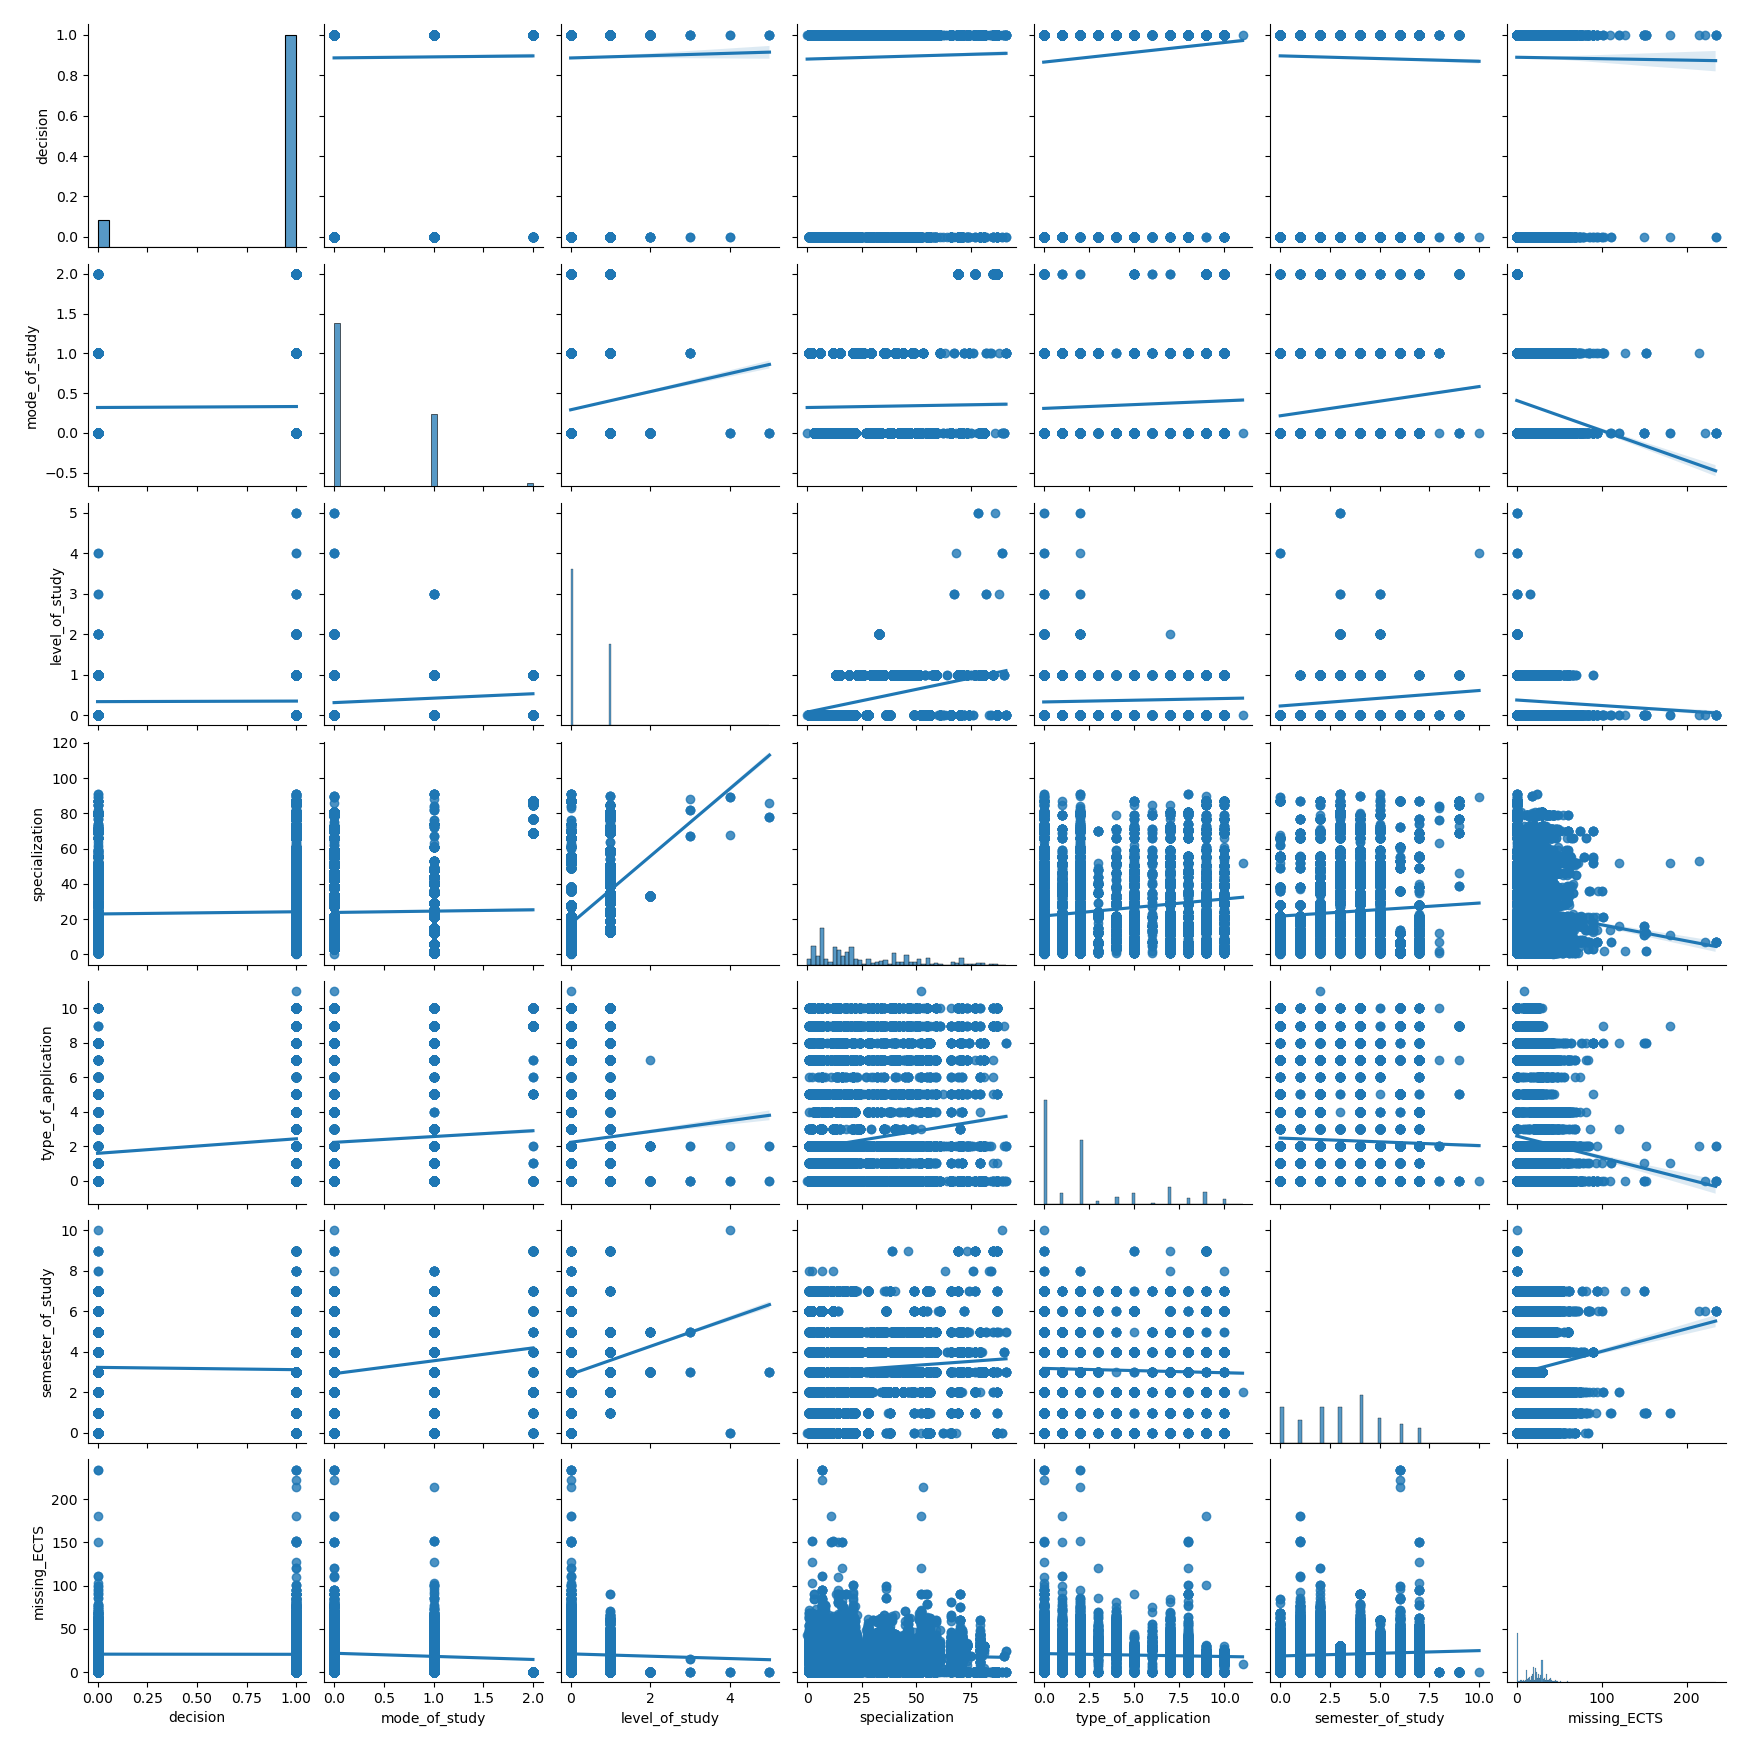
\includegraphics[width=0.5\textwidth]{img/pairplot_selected_columns.png}
    \caption{Pairplot of selected columns in dataset}
    \label{fig:selected_features_pariplot}
\end{figure}

\begin{table}
    \centering
    \caption{Selected features}
    \label{tab:selected_features}
    \begin{tabular}{l}
        \hline
        \textbf{Feature}\\
        \hline
        mode\_of\_study\\
        level\_of\_study\\
        specialization\\
        type\_of\_application\\
        semester\_of\_study\\
        missing\_ECTS\\
        \hline
    \end{tabular}
\end{table}

\begin{figure}
    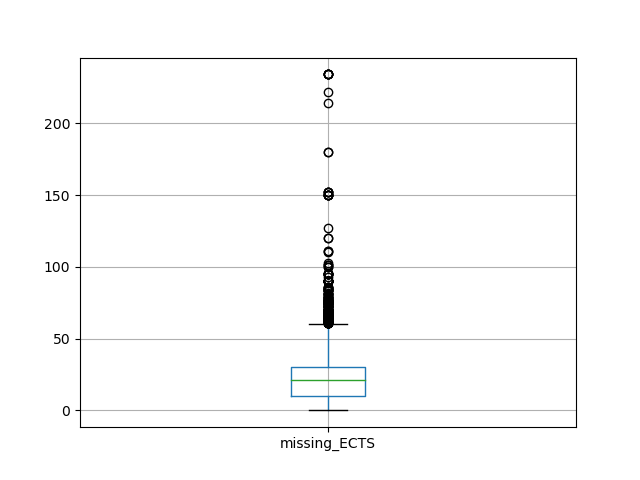
\includegraphics[width=0.5\textwidth]{img/box_missing.png}
    \caption{Boxplot of values in missing\_ECTS column}
    \label{fig:box_missing}
\end{figure}

\begin{figure}
    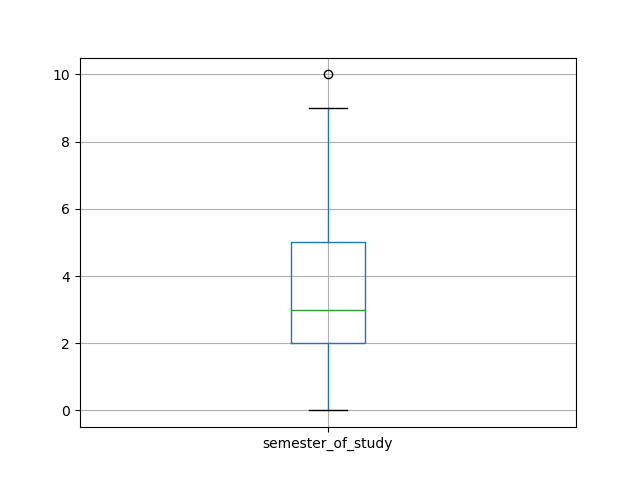
\includegraphics[width=0.5\textwidth]{img/box_semester.png}
    \caption{Boxplot of values in ECTS\_in\_recent\_semester column}
    \label{fig:box_semester}
\end{figure}
